\documentclass[12pt,a4paper]{article}

\usepackage[english]{babel}
\usepackage[utf8x]{inputenc}
\usepackage{amsmath,amssymb}
\usepackage{graphicx}
\usepackage{hyperref}
\usepackage{listings}

\title{Graph Powered Machine Learning - Exercise  1}
\author{J{\"o}rg Schad}

\begin{document}
\maketitle

Thank you for participating in the Graph Powered Machine Learning Workshop! This is the first of two Exercises.

\section*{Logistics}

\begin{itemize}
  \item You can submit into groups up-to 4 people, please include: 
  \begin{itemize}
  \item Full Name
  \item Student ID and Affiliation
  \item Email Address
  \end{itemize} for all group members
  \item Deadline: October 2nd, 23:59 CET
  \item Submit to joerg@arangodb.com
  \item Code can be either submitted in .py file or as .ipynb notebook (will give you the chance to add additional information)
  \item Feel free to use existing notebooks as starting point

\end{itemize}


\section{Property Graph vs RDF/SPARQL}
Recall the Train Network from the \href{https://colab.research.google.com/github/joerg84/Graph_Powered_ML_Workshop/blob/master/Graphs_Queries.ipynb#scrollTo=UR9vgfDa-8_n}{Graph Query Notebook.}  

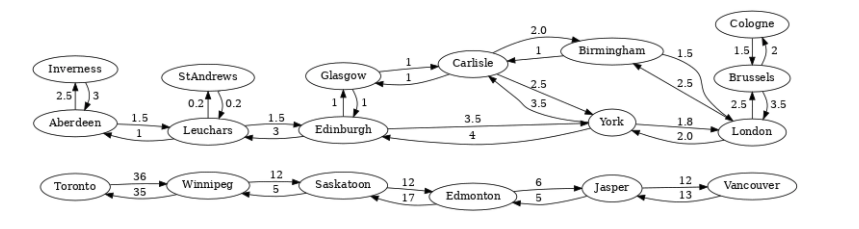
\includegraphics[scale=0.5]{Exercise_1/train_network.png}

Using \href{https://rdflib.readthedocs.io/en/stable/index.html}{rdflib} (e.g.,\href{https://colab.research.google.com/github/joerg84/Graph_Powered_ML_Workshop/blob/master/Sparql.ipynb}{RDF and SPARQL Notebook}
\begin{enumerate}
    \item Create an RDF Graph representing the same road network and travel times
    \item Implement a SPARQL query returning all cities which can be reached from London. Bonus: all cities which can be reached within less than 5 hours. Hint: You might want to consider \href{https://www.w3.org/TR/sparql11-property-paths/}{property paths}.
    \item Implement generic python code (i.e., the algorithms don't have to be specified in SPARQL, but could be) for the Single Source Shortest Path algorithm and return the shortest paths to all other cities starting from London. You can choose either Dijkstra's or Bellman-Ford's algorithm.
\end{enumerate}


\section{Pagerank}
\lstset{language=Python}
For a given directed networkx Graph (e.g., 
\lstinline"G = nx.DiGraph(nx.path_graph(4)") write a PageRank algorithm using python from scratch (i.e., don't use nx.pagerank()).
Your PageRank algorithm should consider a parameter alpha, representing the damping factor and return a dictionary of nodes with their PageRank as value.

\end{document}